\section{Traffic predictive model validation on Italian Internet provider network}

{In addition to the validation of our predictive models of the incoming traffic over the Mininet environment, the accuracy has been also tested on data measured from a real network device (Ubiquiti EP-16) of an Italian internet internet provider (Sonicatel S.r.l.). Data collection has been performed using the software Cacti \cite{Cacti}.\\
Since this device is part of a running commercial network, some constraints in data collection have forced to only measure the sum of all packets entering and leaving the device, and it has been possible to extract from such traffic only incoming VOIP packets: i.e., it has not been possible to extract packets differentiated for each DSCP. Moreover, it is not currently possible to apply any type of closed-loop control on the network device. For the above 2 reasons the control performance validation in the following sections is not based on this real traffic dataset.\\
About data analysis, 53 days of data measurements have been used for RF training and about 3 days for model validation. Figure \ref{fig:{errorPescara}} shows the prediction on three classes of packets: all packets received, all packets transmitted, VOIP packets received. The plots show that our methodology provides a very accurate prediction even on a real internet service provider network.}
\begin{figure}[h!]
	\centering
	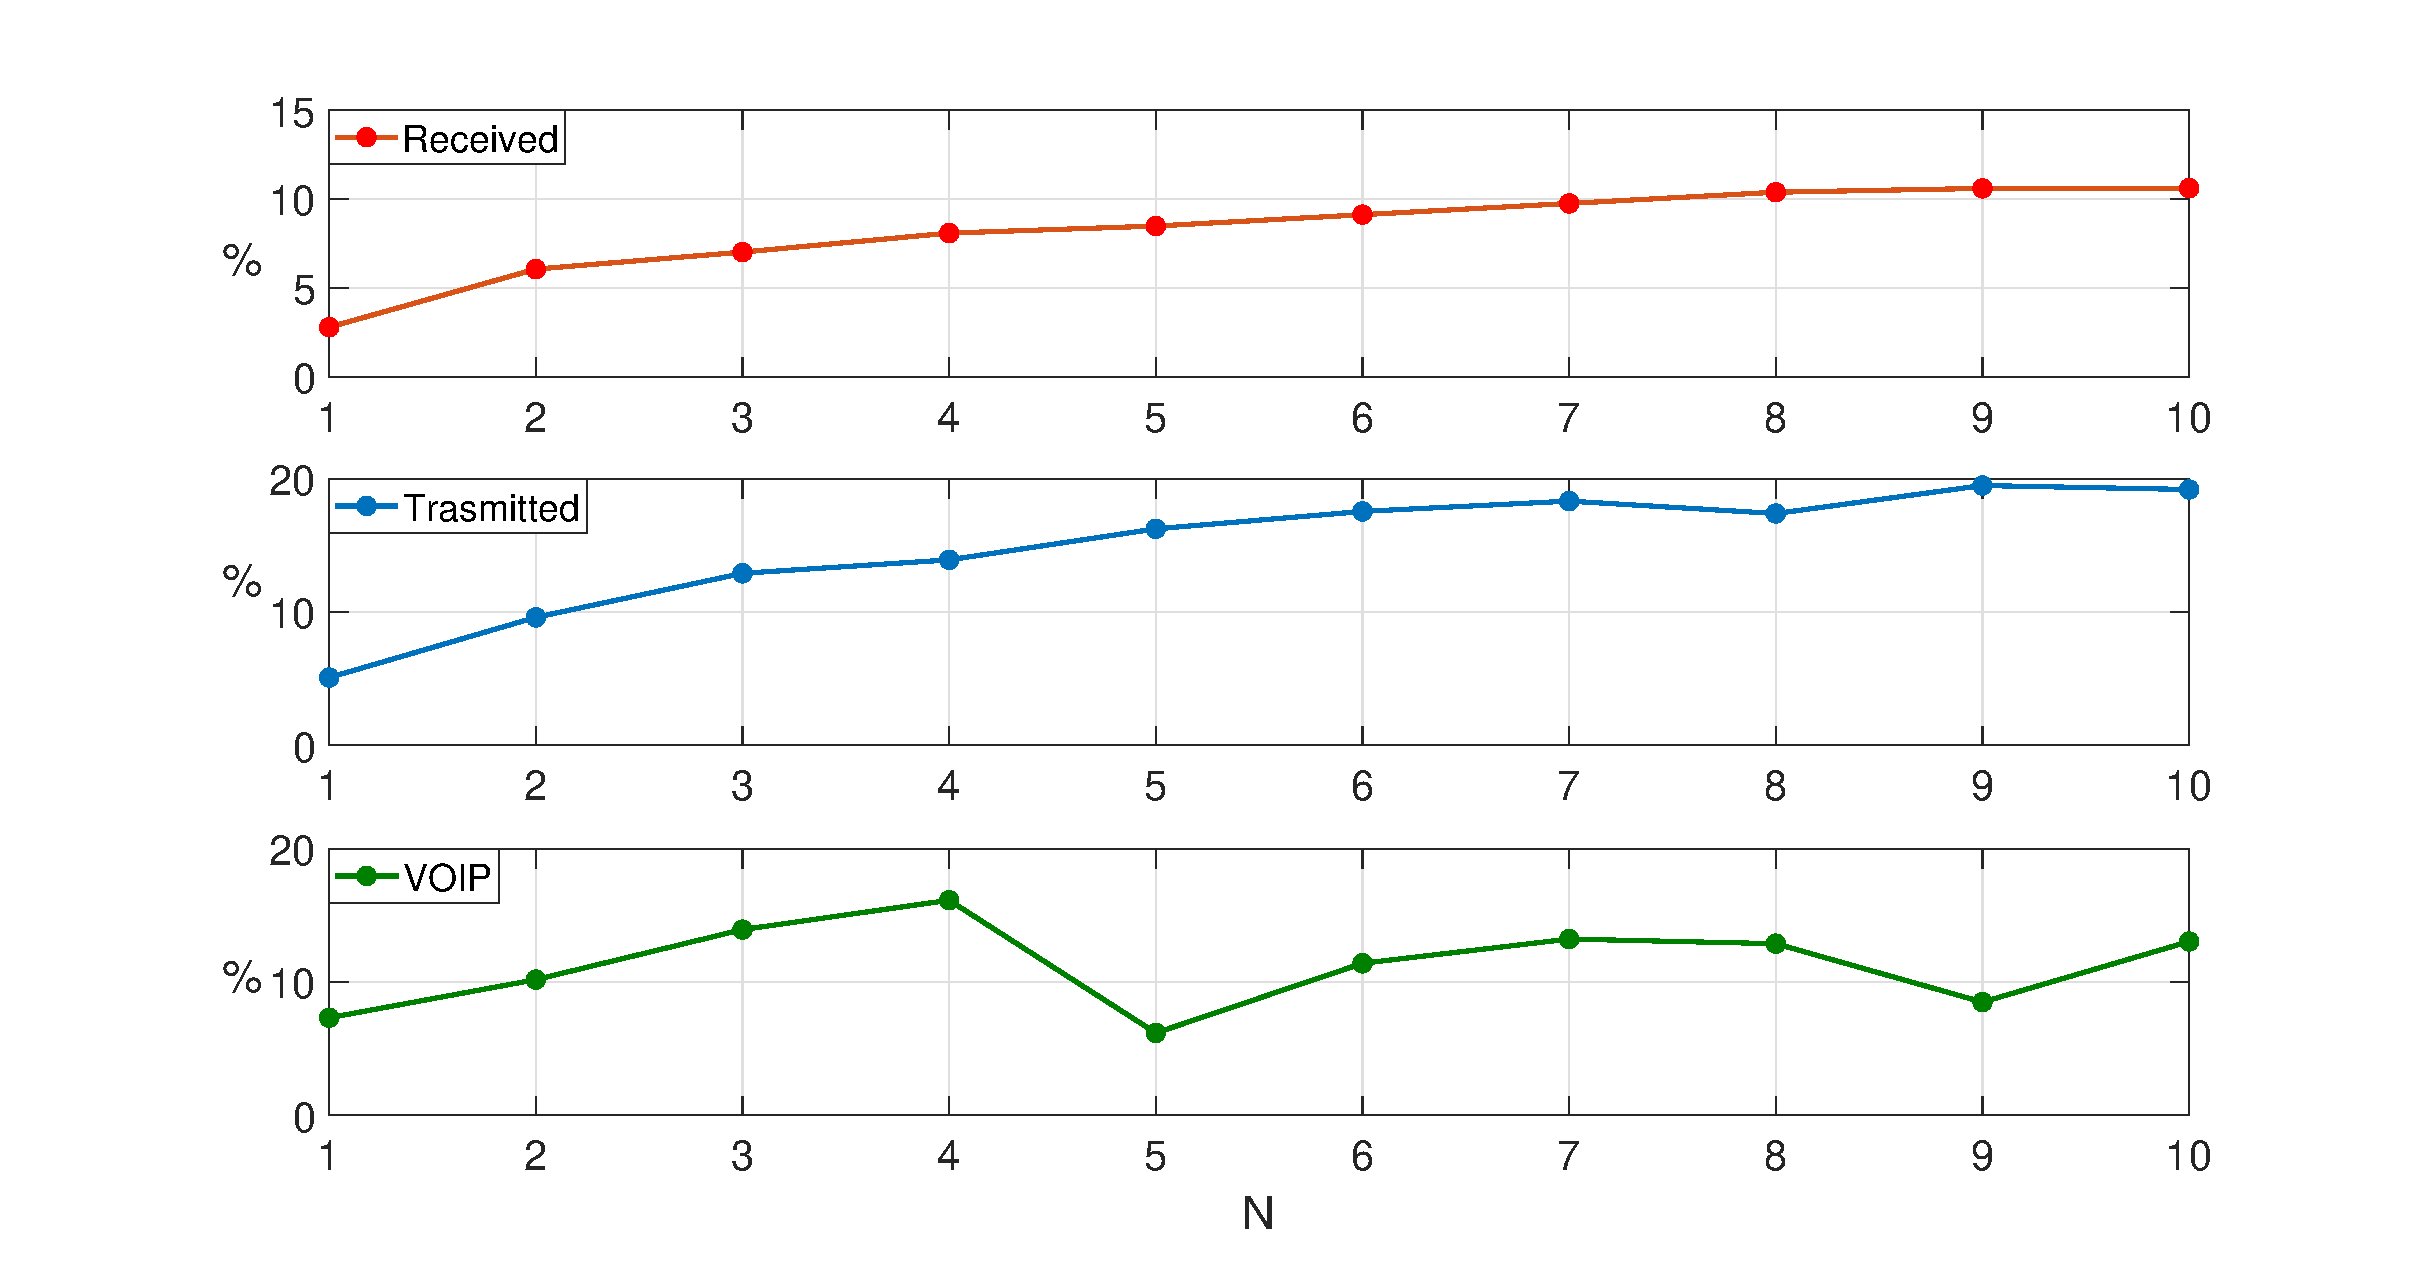
\includegraphics[trim={120 0 120 0}, width=1\linewidth]{figure/Error_PESCARA_DATA.eps}
	\caption{NRMSE of the packets predictive model over a time horizon of $N=10$.}
	\label{fig:{errorPescara}}
\end{figure}

\section{Control performance validation over dedicated hardware network}